% -*- coding: UTF-8 -*-
% vim: autoindent expandtab tabstop=4 sw=4 sts=4 filetype=tex
% chktex-file 27 - disable warning about missing include files

% Main document
% ===========================================================================
% This is part of the document "Project documentation template".
% Authors: brd3, kaa1
%
%---------------------------------------------------------------------------

\documentclass[
    a4paper,                % paper format
    10pt,                   % fontsize
    %twoside,               % double-sided
    openright,              % begin new chapter on right side
    notitlepage,            % use no standard title page
    parskip=half,           % set paragraph skip to half of a line
]{scrreprt}                 % KOMA-script report
%---------------------------------------------------------------------------
\raggedbottom{}
%\KOMAoptions{cleardoublepage=plain}         % Add header and footer on blank pages


% Load Standard Packages:
%---------------------------------------------------------------------------
\usepackage{scrpage2}
\usepackage[ngerman]{babel}                                             % german hyphenation
\usepackage[utf8]{inputenc}                                             % UTF-8 input encoding
\usepackage[T1]{fontenc}                                                % hyphenation of words with ä,ö and ü
\usepackage{textcomp}                                                   % additional symbols
\usepackage{etoolbox}                                                   % color manipulation of header and footer
\usepackage{graphicx}                                                   % integration of images
\usepackage{float}                                                      % floating objects
\usepackage[font={footnotesize,it}]{caption}                            % for captions of figures and tables
\usepackage{booktabs}                                                  % package for nicer tables
% \usepackage{tabu}                                                       % package for tables
\usepackage{tocvsec2}                                                   % provides means of controlling the sectional numbering
\usepackage[square,sort,comma,authoryear]{natbib}                       % provides various citation styles
\usepackage{wrapfig}                                                    % provides floating of text around images
\usepackage{nameref}                                                    % provides printing names of references
\usepackage{colortbl}                                                   % Colored tables
\usepackage{scrhack}                                                    % Remove float errors and warnings
\usepackage{pgfgantt}                                                   % Provides GANTT charts
\usepackage{array}
%---------------------------------------------------------------------------

% Load Math Packages
%---------------------------------------------------------------------------
\usepackage[fleqn]{amsmath}                                             % various features to facilitate writing math formulas
\usepackage{amsthm}                                                     % enhanced version of latex's newtheorem
\usepackage{amsfonts}                                                   % set of miscellaneous TeX fonts that augment the standard CM
\usepackage{amssymb}                                                    % mathematical special characters
\usepackage{exscale}                                                    % mathematical size corresponds to textsize
%---------------------------------------------------------------------------

% Package to facilitate placement of boxes at absolute positions
%---------------------------------------------------------------------------
\usepackage[absolute]{textpos}
\setlength{\TPHorizModule}{1mm}
\setlength{\TPVertModule}{1mm}
%---------------------------------------------------------------------------

% PDF as attachment
%---------------------------------------------------------------------------
\usepackage{pdfpages}
%---------------------------------------------------------------------------

% Definition of Colors
%---------------------------------------------------------------------------
\RequirePackage{color}                          % Color (not xcolor!)
\definecolor{linkblue}{rgb}{0,0,0.8}            % Standard
\definecolor{darkblue}{rgb}{0,0.08,0.45}        % Dark blue
\definecolor{bfhgrey}{rgb}{0.41,0.49,0.57}      % BFH grey
%\definecolor{linkcolor}{rgb}{0,0,0.8}              % Blue for the web- and cd-version!
\definecolor{linkcolor}{rgb}{0,0,0}                 % Black for the print-version!
\colorlet{Black}{black}

%---------------------------------------------------------------------------

% Load listings package
% which provides source code formatting
%---------------------------------------------------------------------------
\usepackage{listings}                                                   % provides source code formatting
% Define XML colors
\lstdefinelanguage{XML}
{
  basicstyle=\ttfamily\footnotesize,
  morestring=[b]'',
  moredelim=[s][\bfseries\color{maroon}]{<}{\ },
  moredelim=[s][\bfseries\color{maroon}]{</}{>},
  moredelim=[l][\bfseries\color{maroon}]{/>},
  moredelim=[l][\bfseries\color{maroon}]{>},
  morecomment=[s]{<?}{?>},
  morecomment=[s]{<!--}{-->},
  commentstyle=\color{codecommentcolor},
  stringstyle=\color{darkblue},
  identifierstyle=\color{red}
}
% Change captions of listings
\renewcommand{\lstlistingname}{Auflistung}
\renewcommand{\lstlistlistingname}{Auflistungsverzeichnis}
%---------------------------------------------------------------------------

% Hyperref Package (Create links in a pdf)
%---------------------------------------------------------------------------
\usepackage[
    pdftex,ngerman,bookmarks,plainpages=false,pdfpagelabels,
    backref = {false},                                      % No index backreference
    colorlinks = {true},                  % Color links in a PDF
    hypertexnames = {true},               % no failures "same page(i)"
    bookmarksopen = {true},               % opens the bar on the left side
    bookmarksopenlevel = {0},             % depth of opened bookmarks
    pdftitle = {Volume ray casting --- basics \& principles},      % PDF-property
    pdfauthor = {Sven Osterwalder},                           % PDF-property
    pdfsubject = {Volume ray casting},        % PDF-property
    linkcolor = {linkcolor},              % Color of Links
    citecolor = {linkcolor},              % Color of Cite-Links
    urlcolor = {linkcolor},               % Color of URLs
]{hyperref}
%---------------------------------------------------------------------------

% Geometry package: Set up page dimension
%---------------------------------------------------------------------------
\usepackage[a4paper,
    left=25mm,
    right=25mm,
    top=27mm,
    headheight=20mm,
    headsep=10mm,
    textheight=242mm,
    footskip=15mm
]{geometry}
%---------------------------------------------------------------------------

% Makeindex Package
%---------------------------------------------------------------------------
\usepackage{makeidx}                                % To produce index
\makeindex                                      % Index-Initialisation
%---------------------------------------------------------------------------

% Glossary Package
%---------------------------------------------------------------------------
% the glossaries package uses makeindex
% if you use TeXnicCenter do the following steps:
%  - Goto "Ausgabeprofile definieren" (ctrl + F7)
%  - Select the profile "LaTeX => PDF"
%  - Add in register "Nachbearbeitung" a new "Postprozessoren" point named Glossar
%  - Select makeindex.exe in the field "Anwendung" ( ..\MiKTeX x.x\miktex\bin\makeindex.exe )
%  - Add this [ -s "%tm.ist" -t "%tm.glg" -o "%tm.gls" "%tm.glo" ] in the field "Argumente"
%
% for futher informations go to http://ewus.de/tipp-1029.html
%---------------------------------------------------------------------------
\usepackage[nonumberlist]{glossaries}
%\usepackage[xindy,nonumberlist]{glossaries}
\newglossaryentry{OWL}{name={OWL},description={
    Web Ontology Language;
    Ontologiesprache für das semantische Web.
    Mit dieser Sprache können Ontologien beschrieben werden.
}}

\makeglossaries{}
%---------------------------------------------------------------------------

% Fancyrb package
%---------------------------------------------------------------------------
\usepackage{fancyvrb}
\RecustomVerbatimCommand{\VerbatimInput}{VerbatimInput}
{fontsize=\footnotesize,
    %
    frame=lines,  % top and bottom rule only
    framesep=2em, % separation between frame and text rulecolor=\color{Gray},
    %
    label=\fbox{\color{Black}},
    labelposition=topline,
    %
    commandchars=\|\(\), % escape character and argument delimiters for
    % commands within the verbatim
    % commentchar=*        % comment character
}
%---------------------------------------------------------------------------

% TODO notes package
%---------------------------------------------------------------------------
\usepackage[textwidth=65mm]{todonotes}
%---------------------------------------------------------------------------

% Intro:
%---------------------------------------------------------------------------
%\begin{document}                                % Start Document
\settocdepth{section}                                                       % Set depth of toc
\pagenumbering{roman}                                                       
%---------------------------------------------------------------------------

\providecommand{\titel}{Volume ray casting --- basics \& principles}
                  % Titel der Arbeit aus Datei titel.tex lesen
% -*- coding: UTF-8 -*-
% vim: autoindent expandtab tabstop=4 sw=4 sts=4 filetype=tex
% chktex-file 27

\providecommand{\versionnumber}{0.1}		%  Hier die aktuelle Versionsnummer eingeben
\providecommand{\versiondate}{{\today}}		%  Hier das Datum der aktuellen Version eingeben
                % Versionsnummer und -datum aus Datei version.tex lesen

% Set up header and footer
%---------------------------------------------------------------------------

\deftripstyle{newlayout}
  [0pt] % no header line
  [0pt] % no footer line
  {}
  {}
  {}
  {\color{bfhgrey} \footnotesize \titel, Version \versionnumber, \versiondate}
  {}
  {\color{bfhgrey} \thepage}

\pagestyle{newlayout}
% use "pagestyle" also on chapter starting pages 
\renewcommand{\chapterpagestyle}{newlayout}
\renewcommand{\chaptermark}[1]{\markboth{\thechapter.  #1}{}}
\renewcommand*{\headfont}{\normalfont}
\renewcommand*{\footfont}{\normalfont}
%---------------------------------------------------------------------------

% We need this as mr. gantt chart (teh package..) thinks text should be gray..
\color{black}

\begin{document}

% Title Page and Abstract
%---------------------------------------------------------------------------
% -*- coding: UTF-8 -*-
% vim: autoindent expandtab tabstop=4 sw=4 sts=4 filetype=tex
% chktex-file 27 - disable warning about missing include files
% chktex-file 36 - disable put space in front of parentheses warning

\begin{titlepage}

    % BFH-Logo absolute placed at (28,12) on A4 and picture (16:9 or 15cm x 8.5cm)
    % Actually not a realy satisfactory solution but working.
    %---------------------------------------------------------------------------
    \setlength{\unitlength}{1mm}
    \begin{textblock}{20}[0,0](28,12)
        
\includegraphics[scale=1.0]{img/BFH_Logo_B.png}
    \end{textblock}

    \begin{textblock}{154}(28,48)
        \begin{picture}(150,2)
            \put(0,0){\color{bfhgrey}\rule{150mm}{2mm}}
        \end{picture}
    \end{textblock}

    \begin{textblock}{154}[0,-0.2](26,40)
        \centering
        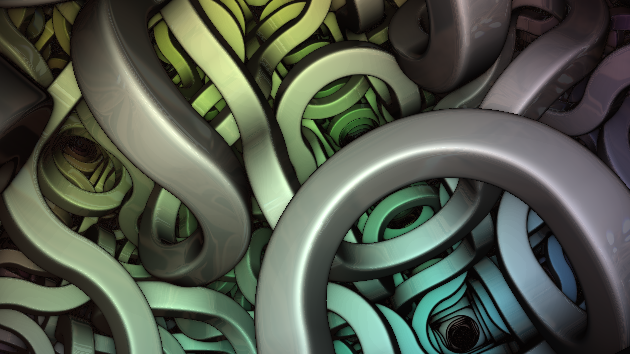
\includegraphics[scale=0.6]{img/logo.png}
    \end{textblock}

    \begin{textblock}{154} (28,135)
        \begin{picture}(150,2)
            \put(0,0){\color{bfhgrey}\rule{150mm}{2mm}}
        \end{picture}
    \end{textblock}
    \color{black}

    \begin{flushleft}
        \vspace*{120mm}
        \fontsize{26pt}{28pt}\selectfont
        \titel{}\\
        \vspace{3mm}
        \fontsize{14pt}{16pt}\selectfont
        \textbf{Projektarbeit 1} \\
        \vspace{6mm}

        \textbf{MTE7101} \\
        \vspace{3mm}

        \begin{textblock}{150} (28,215)
            \fontsize{10pt}{17pt}\selectfont
            \begin{tabbing}
            xxxxxxxxxxxxxxx   \= xxxxxxxxxxxxxxxxxxxxxxxxxxxxxxxxxxxxxxxxxxxxxxx \kill
            Studiengang:      \> Informatik                                         \\
            Autor:            \> Sven Osterwalder\protect\footnotemark[1]{}         \\
            Betreuer:         \> Prof.~Claude Fuhrer\protect\footnotemark[2]{} \\
            Datum:            \> \vhCurrentDate{}\\
            Version:          \> \vhCurrentVersion\\
            \end{tabbing}
        \end{textblock}
    \end{flushleft}
    \footnotetext[1]{sven.osterwalder@students.bfh.ch}
    \footnotetext[2]{claude.fuhrer@bfh.ch}

    \begin{textblock}{150} (28,280)
        \noindent
        \color{bfhgrey}\fontsize{9pt}{10pt}\selectfont
        Berner Fachhochschule | Haute école spécialisée bernoise | Bern University of Applied Sciences
        \color{black}\selectfont
    \end{textblock}

    \vfill
    
\includegraphics[height=\baselineskip]{img/by-sa}\\ \small{\sffamily{Licensed under the Creative Commons Attribution-ShareAlike 3.0 License}}

\end{titlepage}
          % activate for Titelseite mit Bild
\cleardoublepage{}
\phantomsection{}
% -*- coding: UTF-8 -*-
% vim: autoindent expandtab tabstop=4 sw=4 sts=4 filetype=tex
% chktex-file 27 - disable warning about missing include files

% Versionenkontrolle :
% -----------------------------------------------

\chapter*{}
\label{chap:versionen}

\begin{versionhistory}
    \vhEntry{0.1}{25.09.2015}{SO}{Initiale Erstellung des Dokumentes}
    \vhEntry{0.2}{27.09.2015}{SO}{Entwickeln einer initialen Struktur,
        Dokumentaufbau, Entwicklung Kapitel~\ref{chap:procedure}, Beschreibung von
        Ray Tracing in Kapitel~\ref{chap:theoretical_background}, Hinzufügen des
        Kapitels~\ref{chap:20_administrative}, Einführen von TODO-Notizen
    }
    \vhEntry{0.3}{29.09.2015}{SO}{Einführen von Meeting
        Minutes~\ref{chap:10_meeting_minutes}, Erweitern des
        Kapitels~\ref{chap:theoretical_background} um Belechtungsmodelle, Beschreiben von
        lokalen Beleuchtungsmodellen
    }
    \vhEntry{0.4}{04.10.2015}{SO}{Hinzufügen von Standards und
        Richtlinien~\ref{subsec:standards_guidelines}, Erweitern des
        Kapitels~\ref{chap:theoretical_background} um globale
        Belechtungsmodelle~\ref{subsec:global_illumination_models} sowie Ray
        Casting~\ref{subsec:ray_casting}, Entfernen der Schriftart `cmbright', Hinzufügen
        des Kapitels über (implizite) Oberflächen~\ref{sec:surfaces}
    }
    \vhEntry{0.5}{11.10.2015}{SO}{Neuordnung des
        Kapitels~\ref{chap:theoretical_background}: Hinzufügen des Kapitels über Ray
        Tracing~\ref{sec:ray_casting_tracing} sowie über Darstellung von impliziten
        Oberflächen~\ref{sec:description_implicit_surfaces}
    }
    \vhEntry{0.6}{14.10.2015}{SO}{Hinzufügen von TODO-Notizen, Anpassung der
        Textdarstellung in Formeln
    }
    \vhEntry{0.7}{16.10.2015}{SO}{Hinzufügen einer Illustration des
        Phong-Beleuchtungmodelles in Kapitel~\ref{subsec:local_illumination_models},
        Abarbeiten von TODO-Notizen in diversen Kapiteln, Erweitern des Kapitels über
        (implizite) Oberflächen~\ref{sec:surfaces}
    }
    \vhEntry{0.8}{17.10.2015}{SO}{Hinzufügen einer Illustration des Ray Tracing
        Algorithmus in Kapitel~\ref{subsec:global_illumination_models}
    }
    \vhEntry{0.9}{19.10.2015}{SO}{Beginn Kapitel über Rendering von impliziten
        Oberflächen~\ref{sec:rendering_implicit_surfaces}
    }
    \vhEntry{0.10}{21.10.2015}{SO}{Erweiterung Kapitel über Rendering von
        impliziten Oberflächen, Einführung Kapitel über die Umsetzung eines
        Prototypen~\ref{chap:prototype}
    }
    \vhEntry{0.11}{24.10.2015}{SO}{Umstrukturierung des Dokumentes, Anpassung
        der Dokumentvorlage, Nachführen der Versionshistorie, Ausführen der
        Meeting Minutes vom 18.10.2015, Erstellen der Vorlage für Meeting
        Minutes vom 25.10.2015
    }
    \vhEntry{0.12}{31.10.2015}{SO}{Nachführen der Versionshistorie, Ausführen der
        Meeting Minutes vom 25.10.2015, Erstellen der Vorlage für Meeting
        Minutes vom 02.11.2015, Erweiterung des
        Kapitels~\ref{chap:prototype}, Abarbeiten von TODO-Notizen
    }
    \vhEntry{0.13}{07.11.2015}{SO}{Ausführen der Meeting Minutes vom
        02.11.2015, Erweiterung des Kapitels~\ref{chap:prototype}
    }
    \vhEntry{0.14}{15.11.2015}{SO}{Erarbeiten des
        Kapitels~\ref{sec:rendering_implicit_surfaces_shadows},
        Erweiterung des Kapitels~\ref{chap:prototype} um weiche Schatten, 
        Erstellen und Hinzufügen von Bildmaterial zu Kapiteln~\ref{subsec:ray_marching}
        und~\ref{subsec:sphere_tracing}.
    }
    \vhEntry{0.15}{29.11.2015}{SO}{Komplette Überarbeitung des Bildmaterials zu
        Kapiteln~\ref{subsec:ray_marching} und~\ref{subsec:sphere_tracing}.
    }
    \vhEntry{0.16}{06.12.2015}{SO}{Nachführen von Meeting Minutes und der
        Versionierung. Überarbeiten des Zeitplanes, weiter Überarbeitung des
        Bildmaterials. Hinzufügen des Kapitels~\ref{sec:shading}, Hinzufügen
        einer Einleitung zu Kapitel~\ref{chap:theoretical_background}.
    }
\end{versionhistory}

\phantomsection{}
\cleardoubleemptypage{}
\listoftodos{}
\phantomsection{}
\cleardoubleemptypage{}
\setcounter{page}{1}
\cleardoublepage{}
\phantomsection{}
\addcontentsline{toc}{chapter}{Management Summary}
% -*- coding: UTF-8 -*-
% vim: autoindent expandtab tabstop=4 sw=4 sts=4 filetype=tex
% chktex-file 27

\chapter*{Management Summary}
\label{chap:managementSummary}

Lorem ipsum dolor sit amet, consectetur adipiscing elit. Phasellus scelerisque, leo sed iaculis ornare, mi leo semper urna, ac elementum libero est at risus. Donec eget aliquam urna. Lorem ipsum dolor sit amet, consectetur adipiscing elit. Nunc fermentum nunc sollicitudin leo porttitor volutpat. Duis ac enim lectus, quis malesuada lectus. Aenean vestibulum suscipit justo, in suscipit augue venenatis a. Donec interdum nibh ligula. Aliquam vitae dui a odio cursus interdum quis vitae mi. Phasellus ornare tortor fringilla velit accumsan quis tincidunt magna eleifend. Praesent nisl nibh, cursus in mattis ac, ultrices ac nulla. Nulla ante urna, aliquet eu tempus ut, feugiat id nisl. Nunc sit amet mauris vitae turpis scelerisque mattis et sed metus. Aliquam interdum congue odio, sed semper elit ullamcorper vitae. Morbi orci elit, feugiat vel hendrerit nec, sollicitudin non massa. Quisque lacus metus, vulputate id ullamcorper id, consequat eget orci.

\cleardoubleemptypage{}
%---------------------------------------------------------------------------

% Make sure Umlauts are getting displayed correctly.
\lstset{literate=%
    {Ö}{\textcolor{black}{\"O}}1
    {Ä}{{\"A}}1
    {Ü}{{\"U}}1
    {ß}{{\ss}}1
    {ü}{{\"u}}1
    {ä}{{\textcolor{black}{\"a}}}1
    {ö}{{\textcolor{black}{\"o}}}1
    {~}{{\textasciitilde}}1
    {?}{{\textcolor{black}{?}}}1
}

% Table of contents
%---------------------------------------------------------------------------
\tableofcontents
\cleardoublepage{}
%---------------------------------------------------------------------------

% Main part:
%---------------------------------------------------------------------------
\pagenumbering{arabic}
% -*- coding: UTF-8 -*-
% vim: autoindent expandtab tabstop=4 sw=4 sts=4 filetype=tex
% chktex-file 27 - disable warning about missing include files

\chapter{Einleitung}
\label{chap:10_introduction}

Seit dem Bestehen moderner Computer existiert auch die Computergrafik. Ziel der Computergrafik ist es unter Anderem den dreidimensionalen Raum auf eine zweidimensionale Fläche abzubilden, da die Ausgabe meist auf den zweidimensionalen Raum limitiert ist.

Dabei wird zwischen statischen Bildern und dynamischen Bildern unterschieden. Statische Bilder werden bei Bedarf dargestellt und ändern sich in der Regel nicht. Dynamische Bilder können sich hingegen ständig ändern und müssen --- bedingt durch das menschliche Auge --- mit 25 Bildern pro Sekunde ausgegeben werden. Es bestand bereits früh das Bestreben möglichst eine realistische Darstellung zu erhalten. Eine Darstellung also, die möglichst nahe an der menschlichen Wahrnehmung liegt.

Im Laufe der Zeit entstanden verschiedene Ansätze um eine solche Darstellung zu bieten. Ein Teilgebiet davon sind Beleuchtungsmodelle, welche die Beleuchtung einer Darstellung bzw.\ einer Szene berechnen. Dabei wird zwischen lokalen und globalen Beleuchtungsmodellen unterschieden.

Ein globales Beleuchtungsmodell ist Ray Tracing (zu deutsch Strahlenverfolgung), welches 1980 von Turner Whitted vorgestellt wurde wurde. Das Verfahren besticht durch seine Einfachheit und bietet dabei eine hohe Bildqualität mit perfekten Spiegelungen und Transparenzen. Mit entsprechenden Optimierungen ist das Verfahren auch relativ schnell.

Mit schnell ist dabei die Zeit gemeint, die benötigt wird um ein einzelnes Bild darzustellen. Möchte man jedoch eine Darstellung in Echtzeit erreichen, so war das Verfahren lange zu langsam.

Im Rahmen der Weiterentwicklung der Computer und vor allem durch die Weiterentwicklung der Grafikkarten (GPUs) ist Ray Tracing jedoch wieder in den Fokus der Darstellung von Szenen in Echtzeit gerückt.

Diese Projektarbeit stellt ein spezielles, auf Ray Tracing basierendes Verfahren zur Darstellung eines Bildes in Echtzeit vor: Das so Volume Ray Casting oder Sphere Tracing genannte Verfahren.

% -*- coding: UTF-8 -*-
% vim: autoindent expandtab tabstop=4 sw=4 sts=4 filetype=tex
% chktex-file 27 - disable warning about missing include files

\chapter{Administratives}
\label{chap:20_administrative}

\section{Beteiligte Personen}
\label{sec:involved_persons}

\section{Aufbau des Dokumentes}
\label{sec:document_structure}

\section{Ergebnisse}
\label{sec:deliverables}

% -*- coding: UTF-8 -*-
% vim: autoindent expandtab tabstop=4 sw=4 sts=4 filetype=tex
% chktex-file 27 - disable warning about missing include files

\chapter{Aufgabenstellung}
\label{chap:scope}

\section{Motivation}
\label{sec:motivation}

\todo[inline]{Describe motivation}

\subsection{Demoszene}
\label{subsec:demoscene}

\todo[inline]{Loose some words about demoscene! }

\section{Ziele und Abgrenzung}
\label{sec:objectives}

\todo[inline]{Describe objectives}

\subsection{Vorgängige Arbeiten}
\label{subsec:preliminaries}

\todo[inline]{Describe preliminaries}

\subsection{Neue Lerninhalte}
\label{subsec:new_learning_contents}

\todo[inline]{Describe new learning contents}

% -*- coding: UTF-8 -*-
% vim: autoindent expandtab tabstop=4 sw=4 sts=4 filetype=tex
% chktex-file 27 - disable warning about missing include files

\chapter{Vorgehen}
\label{chap:procedure}

\section{Arbeitsorganisation}
\label{sec:organization}

\subsection{Regelmässige Treffen}
\label{subsec:meetings}

Regelmässige Besprechungen mit dem Betreuer der Arbeit halfen die gesteckten Ziele zu erreichen und Fehlentwicklungen zu vermeiden. Der Betreuer unterstützte den Autor dabei mit Vorschlägen. Die Treffen fanden mindestens alle zwei Wochen statt, sie wurden in Form eines Protokolles festgehalten.

\section{Projekphasen}
\label{sec:project_schedule}

\subsection{Meilensteine}
\label{subsec:milestones}

Um bei der Arbeit ein möglichst strukturiertes Vorgehen einzuhalten, wurden folgende Projektphasen gewählt:
\begin{itemize}
    \item Projektstart
    \item Erarbeitung und Festhalten der Anforderungen
    \item Erarbeitung der theoretischen Grundlagen
    \item Erstellung der abschliessenden Dokumentation
\end{itemize}

Die Phasen der Erarbeitung der theoretischen Grundlagen sowie die Erstellung der abschliessenden Dokumentation liefen parallel ab.

\subsection{Zeitplan / Projektphasen}
\label{subsec:timeschedule}

\begin{figure}[H]
    \begin{ganttchart}[
        vgrid,
        x unit=0.7cm,
        bar/.append style={fill=bfhgrey!50},
    ]{1}{16}
        \gantttitle{2015}{14}
        \gantttitle{2016}{2} \\
        \gantttitlelist{1,...,16}{1} \\ % chktex 11: Disable "you should use \ldots to achieve.."
        \ganttbar{Projektstart}{1}{1} \\
        \ganttlinkedbar{Anforderungen}{2}{3} \ganttnewline{}
        \ganttbar{Erarbeitung theoretische Grundlagen}{2}{12} \\
        \ganttbar{Dokumentation}{1}{2} \ganttbar{}{1}{16} \\
        \ganttbar{Präsentation/Verteidigung vorbereiten}{15}{16}
    \end{ganttchart}
    \caption{Zeitplan; Der Titel stellt Jahreszahlen, der Untertitel Semesterwochen dar}
\end{figure}
\todo[inline]{Update schedule}
\todo[inline]{Add deadline for rough draft for end ov nov / beginning
    of dec}

\subsubsection{Projektstart}
\label{subsubsec:kick_off}
In der ersten Phase wurden die Meilensteine der Arbeit identifiziert und skizziert. Um Details der Aufgabe zu verstehen, wurde das notwendige Vorwissen über globale Beleuchtungsalgorithmen erarbeitet. Weiter wurde das Grundgerüst dieser Dokumentation erstellt.

\subsubsection{Anforderungen}
\label{ssubsec:requirements}
In dieser Phase wurde das Ziel dieser Projektarbeit festgelegt. Vom Ziel ausgehend wurden die dazu erforderlichen Projektphasen festgelegt.

\subsubsection{Erarbeitung theoretische Grundlagen}
\label{ssubsec:theoretical_background}
\todo[inline]{Describe theoretical background}

\subsubsection{Dokumentation}
\label{ssubsec:documentation}

Die vorliegende Arbeit entspricht der Dokumentation. Sie wurde während der gesamten Projektarbeit stetig erweitert und diente zur Reflexion von fertiggestellten Teilen.

\section{Technologien}
\label{sec:technologies}

\subsection{Tools und Software}
\label{subsec:tools_software}

\noindent\emph{Dokumentation}
\begin{description}
    \item[\LaTeX] Eine Makro-Sammlung für das \TeX-System. Wurde zur Erstellung
        dieser Dokumentation eingesetzt. Diese Dokumentation wurde mittels \LaTeX{} geschrieben.
    \item[Make] Build-Automations-Werkzeug, wurde zur Erstellung dieses Dokumentes eingesetzt.
    \item[zotero] Ein freies, quelloffenes Literaturverwaltungsprogramm zum Sammeln, Verwalten und Zitieren unterschiedlicher Online- und Offline-Quellen~\cite{wikipedia_foundation_zotero_2015}.
    \item[VIM] Vi IMproved. Ein freier, quelloffener Texteditor zur Textbearbeitung.
\end{description}

\noindent\emph{Arbeitsorganisation}
\begin{description}
    \item[Git] Freie Software zur verteilten Versionsverwaltung, wurde für die
        Entwicklung dieser Dokumentation verwendet. Die Projektarbeit findet sich
        unter~\href{https://www.github.com/sosterwalder/mte7101-project1}{GitHub}\footnote{\href{https://www.github.com/sosterwalder/mte7101-project1}{https://www.github.com/sosterwalder/mte7101-project1}}.
    \item[GitHub] Eine freie Hosting-Platform für Git mit Weboberfläche.
\end{description}

\subsection{Standards und Richtlinien}
\label{subsec:standards_guidelines}

\subsubsection{Pseudecode}
\label{ssubsec:standards_guidelines:psuedocode}

Da der Autor dieser Arbeit bedingt durch seine täglich Arbeit mit der Programmiersprache Python relativ bewandert ist, wird daher diese als Sprache zur Beschreibung von Pseudcode verwendet.
Dabei wird aber kein Augenmerk auf die formale Korrektheit, geschweige denn der Lauffähigkeit des Pseudocodes gelegt.

% -*- coding: UTF-8 -*-
% vim: autoindent expandtab tabstop=4 sw=4 sts=4 filetype=tex
% chktex-file 27 - disable warning about missing include files

\chapter{Theoretischer Hintergrund}
\label{chap:theoretical_background}

\section{Beleuchtungsmodelle}
\label{sec:illumination_models}

Sofern nicht anders vermerkt, basiert der folgende Abschnitt auf~\cite{whitted_improved_1980}[S. 343] sowie auf~\cite{hughes_computer_2013}.

Beleuchtungsmodelle beschreiben, wieviel Licht von einem sichtbaren Punkt einer Oberfläche zum Betrachter emitiert wird. In der Regel wird das Licht als Funktion in Abhängigkeit folgender Faktoren beschrieben:
\begin{itemize}
    \item Richtung der Lichtquelle \item Lichstärke
    \item Position des Betrachters
    \item Orientierung der Oberfläche
    \item Oberflächenbeschaffenheit
    \item Globale Umgebung
\end{itemize}

Es wird dabei zwischen lokalen und globalen Belechtungsmodellen unterschieden.

\subsection{Lokale Beleuchtungsmodelle}
\label{subsec:local_illumination_models}

Lokale Beleuchtungsmodelle aggregieren Daten von benachbarten, eben lokalen, Oberflächen. Diese Modelle sind in deren Umfang allerdings limitiert, da sie normalerweise nur Lichtquellen sowie die Orientierung einer Oberfläche einbeziehen. Sie ignorieren dabei aber die globale Umgebung, in welcher sich eine Oberfläche befindet.
Dies ist dadurch bedingt, dass die traditionell verwendeten Algorithmen zur Berechnung der Sichtbarkeit von Oberflächen, über keine globalen Daten verfügen.

Als Beispiel für ein lokales Beleuchtungsmodell dient das Phong-Beleuchtungsmodell, welches von Bui-Tong Phong entwickelt wurde.
Es beschreibt die reflektierte (Licht-) Intensität als Zusammensetzung aus der ambienten, der diffusen und der ideal spiegelnden Reflexion einer Oberfläche:
\begin{equation}
    I = I_{ambient} + I_{diffuse} + I_{specular}
\end{equation}
oder mathematisch ausgedrückt:
\begin{equation}
    I = I_a + k_d \displaystyle\sum_{j=1}^{ls} (\overrightarrow{N} \cdot \overrightarrow{L_j}) + k_s \displaystyle\sum_{j=1}^{ls} (\overrightarrow{N} \cdot \overrightarrow{L_j^`} )
\end{equation}
wobei gilt:
\begin{itemize}
    \item $I$:                      Die reflektierte (Licht-) Intensität
    \item $I_a$:                    Reflektion bedingt durch die Beleuchtung des Raumes
    \item $k_d$:                    Konstante für die diffuse Komponente des reflektierten Lichtes
    \item $\overrightarrow{N}$:     Einheitsnormale der Oberfläche
    \item $\overrightarrow{L_j}$:   Vektor in Richtung der $j$-ten Lichtquelle
    \item $k_s$:                    Koeffizient der spiegelenden Komponente
    \item $\overrightarrow{L_j^`}$: Vektor in der Hälfte zwischen dem Betrachter und der $j$-ten Lichtquelle
    \item $n$:                      Exponent, welcher von der Reflektion der Oberfläche abhängt
    \item $ls$:                     Anzahl Lichtquellen
\end{itemize}

\subsection{Globale Beleuchtungsmodelle}
\label{subsec:global_illumination_models}

Sofern nicht anders vermerkt, basiert der folgende Abschnitt auf~\cite{foley_computer_1996}[S. 775ff]

Globale Beleuchtungsmodelle beschreiben die reflektierte (Licht-) Intensität eines Punktes aufgrund direkter Lichteinstrahlung durch Lichtquellen sowie durch alles Licht, welches diesen Punkt nach Reflektion von bzw. Durchdringen der eigenen oder anderer Oberflächen erreicht.

Bei globalen Beleuchtungsmodellen unterscheidet man zwischen blickwinkelabhängigen Algorithmen, wie etwa Ray Tracing, und zwischen blickwinkelunabhängigen Algorithmen, wie etwa Photon Mapping.

Blickwinkelabhängige Algorithmen verwenden eine Diskretisierung~\todo{view plane} der sichtbaren Fläche um zu entscheiden, an welchen Punkten, in Blickrichtung des Betrachters, die Beleuchtungsberechnung durchgeführt werden soll. Blickwinkelunabhängige Algorithmen hingegen diskretisieren und verarbeiten die Umgebung um genügend Informationen für die Beleuchtungsberechnung zu haben. Dies erlaubt ihnen die Beleuchtungsberechnung an einem beliebigen Punkt aus einer beliebigen Blickrichtung.

Beide Arten von Algorithmen haben jedoch Vor- und Nachteile. So sind blickwinkelabhängige Algorithmen gut geeignet um Spiegelungen, basierend auf der Blickrichtung des Betrachtes, zu berechnen, eignen sich aber weniger um gleichbleibende diffuse Anteile über weiter Flächen eines Bildes zu berechnen. Bei blickwinkelabhängigen Algorithmen verhält es sich genau umgekehrt.

\subsubsection{Renderinggleichung}
\label{ssubsec:rendering_equation}

Die unter~\ref{subsec:global_illumination_models} genannten Verfahren versuchen auszudrücken, wie sich Licht von einem Punkt im Raum zu einem anderen bewegt. Dabei beschreiben sie die Intensität des Lichtes, ausgehend vom ersten Punkt zum zweiten Punkt. Zusätzlich wird die Intensität des Lichtes, ausgehend von allen anderen Punkten, welche den ersten Punkt erreichen, und zum zweiten Punkt emitiert werden, beschrieben.

James (Jim) Kajiya stellte 1986 die so genannte Renderinggleichung auf, welche genau dieses Verhalten beschreibt:
\begin{equation}
    I(x, x') = g(x, x')[\epsilon(x, x') + \int\limits_{s}\rho(x, x', x'')I(x', x'')dx'']
\end{equation}
wobei gilt:

\captionof{table}{Beschreibung der Komponenten der Renderinggleichung nach~\cite{kajiya_rendering_1986}[S. 143]}
\begin{tabular}{ l l }
    $ x', x' und x''   $: & Punkte in der Umgebung                                                                                                  \\
    $ I(x, x')         $: & Lichtintensität von Punkt $x'$ nach Punkt $x$                                                                           \\
    $ g(x, x')         $: & \parbox[t]{14cm}{Ein auf die Geometrie bezogener Term:                                                                  \\
                                 \hspace*{12mm} $0$:     \hspace*{6mm} $x$ und $x'$ verdecken sich                                                  \\
                                 \hspace*{12mm} $1/r^2$: \hspace*{1mm} $x$ und $x'$ sehen sich, wobei $r$ die Distanz zwischen $x$ und $x'$ ist}    \\
    $ \epsilon(x, x')  $: & Intensität des Lichtes, welches von $x'$ nach $x$ emitiert wird                                                         \\
    $ \rho(x, x', x'') $: & Intensität des Lichtes, welches von $x''$ durch die Oberfläche bei $x'$ nach $x$ gestreut wird                          \\
    $ \int\limits_{S}  $: & \parbox[t]{14cm}{Integral über die Vereinigung aller Flächen, daher $ S = \bigcup{S_{i}} $                              \\
                            Dies bedeutet, dass die Punkte $x$, $x'$ und $x''$ über alle Flächen aller Objekte der Szene ``streifen''.              \\
                            Wobei es sich bei $S_{0}$ um eine zusätzliche Fläche handelt, welche als Hintergrund verwendet wird.                    \\
                            $S_{0}$ ist dabei eine Hemisphäre, welche die gesamte Szene umspannt.}                                                  \\
\end{tabular}

\section{Ray Casting}
\label{sec:ray_casting}

Sofern nicht anders vermerkt, basiert der folgende Abschnitt auf~\cite{hughes_computer_2013}[Kapitel 15, S. 387ff].\\
\\
Um ein Bild möglichst realistisch darzustellen muss berechnet werden, wieviel Licht zu jedem Pixel der sichtbaren Bildfläche (also dem Betrachter) transportiert wird. Da Photonen die Energie des Lichtes transportieren, muss man also das physikalische Verhalten dieser simulieren. Es ist allerdings nicht möglich \textit{alle} Photonen zu simulieren, da der Aufwand schlicht zu gross wäre. Daher macht es Sinn nur einige Photonen (exemplarisch) zu betrachten und dann eine Abschätzung des gesamten Lichtes vorzunehmen.\\
\\
Bei \textbf{Ray Casting} handlt es sich grundsätzlich um eine Strategie zur Simulation, wieviel Licht anhand eines (Licht-) Strahles zu der sichtbaren Bildfläche (also dem Betrachter) transportiert wird.

\begin{figure}[H]
    \centering \rotatebox{0}{\scalebox{0.3}[0.3]{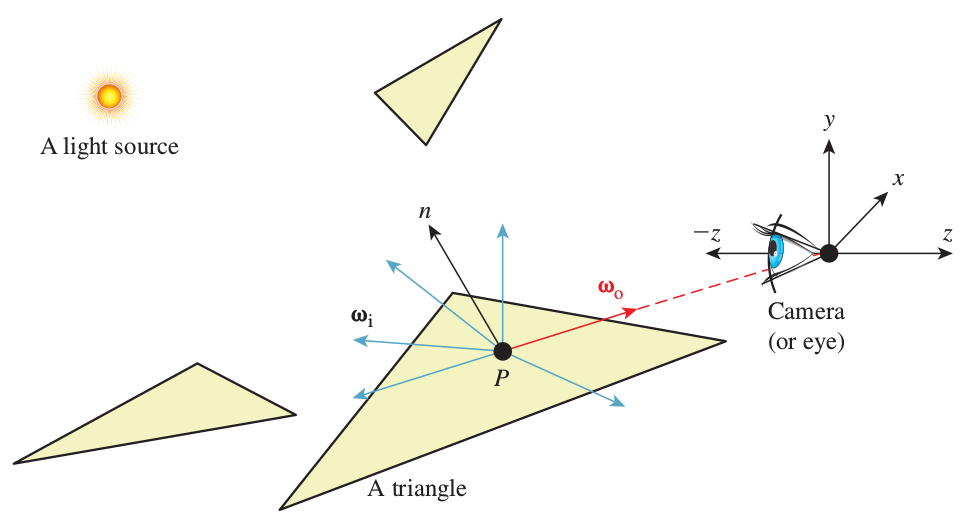
\includegraphics{img/ray_tracing_01.png}}}
    \caption{Punkt $P$ auf einer Oberfläche eines Dreieckes, welcher für die Kamera bzw.\ den Betrachter sichtbar ist.
        Der Betrachter nimmt dabei das Licht, welches aus verschiedenen Richtungen $\omega_{i}$ kommt, über den Punkt $P$ in Richtung $\omega_{0}$ wahr.\label{fig:ray_casting:basics}\protect\footnotemark}
\end{figure}
\footnotetext{Darstellung von~\cite{hughes_computer_2013}[Kapitel 15, Seite 389, Abbildung 15.1]}

Wie in Abbildung~\ref{fig:ray_casting:basics} ersichtlich, gelangt Licht aus vielen Richtungen durch den Punkt $P$ zu dem Betrachter. Dies beinhaltet auch die Möglichkeit, dass
Licht nicht nur von einer Lichtquelle aus, sondern von vielen Lichtquellen aus via $P$ zum Betrachter gelangt. Weiter ist es möglich, dass Licht zuvor an anderen Punkten gestreut
und/oder gespiegelt und erst dann via $P$ zum Betrachter gelangte.\\
\\
Dies führt zu den folgenden Schlussfolgerungen:
\begin{itemize}
    \item Es müssen alle möglichen Richtungen, aus denen Licht kommen könnte, an Punkt $P$ untersucht werden.
    \item Da, bedingt durch technische Limitierungen, nur diskretes Abtasten möglich ist, müssen die Richtungen auf eine endliche Anzahl beschränkt werden, was zu Abtastfehlern führen kann.
\end{itemize}
Um die Abtastfehler zu minieren, können die Richtungen des Abtasten anhand der Lichtquellen priorisiert werden.

\newpage{}

Ein möglicher Algorithmus, wie solch ein Verfahren umgesetzt werden kann, findet sich in~\ref{fig:ray_casting:high_level}.

\begin{python}[caption={Eine abstrakte Umsetzung des Ray Castings.\protect\footnotemark},label={fig:ray_casting:high_level}]
def ray_cast():
    # "pixels" is a list of all pixels of the image plane
    for pixel in pixels:
        # Save all intersections for given pixel
        intersections = []

        # Returns the ray passing through the given
        # pixel from the eye
        ray           = ray_at_pixel(pixel)

        # "scene_triangles" is a list of all triangles
        # coming from meshes contained in the scene to render
        for triangle in scene_triangles:
            p   = intersect(ray, triangle)
            sum = 0

            for light in incoming_lights_at_p:
                sum = sum + l.value
            end

            if is_smallest_intersection(p, intersections):
                pixel = sum
            intersections.append(p)
\end{python}
\footnotetext{Algorithmus in Pseudocode gemäss~\cite{hughes_computer_2013}[Kapitel 15, Seite 391, Auflistung 15.2]}

\newpage{}

\section{Ray Tracing}
\label{sec:ray_tracing}

\todo[inline]{Since illumination returned to the viewer is deter-
mined by a tree of ``rays,'' a ray tracing algorithm is
ideally suited to this model. In an obvious approach to
ray tracing, light rays emanating from a source are traced
through their paths until they strike the viewer. Since
only a few will reach the viewer, this approach is waste-
ful. In a second approach suggested by Appel [1] and
used successfully by MAGI [14], rays are traced in the
opposite direction---from the viewer to the objects in the
scene, as illustrated in Figure 4.
Unlike previous ray tracing algorithms, the visibility
calculations do not end when the nearest intersection of
a ray with objects in the scene is found. Instead, each
visible intersection of a ray with a surface produces more
rays in the /\~ direction, the /5 direction, and in the
direction of each light source. The intersection process is
repeated for each ray until none of the new rays intersects
any object.}

\section{Darstellung impliziter Oberflächen}
\label{sec:implicit_surfaces}

\todo[inline]{Describe implicit surfaces}

% -*- coding: UTF-8 -*-
% vim: autoindent expandtab tabstop=4 sw=4 sts=4 filetype=tex
% chktex-file 27 - disable warning about missing include files

\chapter{Diskussion und Fazit}
\label{chap:discussion_and_conclusion}

\section{Diskussion}
\label{sec:discussion}

\section{Erweiterungsmöglichkeiten}
\label{sec:further_work}

\section{Fazit}
\label{sec:fazit}


%---------------------------------------------------------------------------

% Glossary
%---------------------------------------------------------------------------
\cleardoublepage{}
\phantomsection{}
\addcontentsline{toc}{chapter}{Glossar}
\renewcommand{\glossaryname}{Glossar}
\glsaddall{}
\printglossaries{}
%---------------------------------------------------------------------------

% Bibliography
%---------------------------------------------------------------------------
%\cleardoublepage
\phantomsection{}
\addcontentsline{toc}{chapter}{Literaturverzeichnis}
\bibliographystyle{unsrtnat}
\bibliography{inc/static/bibliography}{}
%---------------------------------------------------------------------------

% Listings
%---------------------------------------------------------------------------
%\cleardoublepage
\phantomsection{}
\addcontentsline{toc}{chapter}{Abbildungsverzeichnis}
\listoffigures
%\cleardoublepage
\phantomsection{}
\addcontentsline{toc}{chapter}{Tabellenverzeichnis}
\listoftables
%\cleardoublepage
\phantomsection{}
\addcontentsline{toc}{chapter}{Auflistungsverzeichnis}
\lstlistoflistings{}
%---------------------------------------------------------------------------

% Index
%---------------------------------------------------------------------------
%\cleardoublepage
%\phantomsection{}
%\addcontentsline{toc}{chapter}{Stichwortverzeichnis}
%\renewcommand{\indexname}{Stichwortverzeichnis}
%\printindex
%---------------------------------------------------------------------------

% Attachment:
%---------------------------------------------------------------------------
%\appendix
\settocdepth{section}
% -*- coding: UTF-8 -*-
% vim: autoindent expandtab tabstop=4 sw=4 sts=4 filetype=tex
% chktex-file 27

% In den Anhang fügen Sie ein:
%  * Details des Projektpans, falls vorhanden
%  * Resultate und Zwischenresultate in Funktion der Projektiterationen
%  * Pflichtenheft / Anforderungsspezifikation (Stand Ende dritter Woche)
%  * Angaben zum Projektrepository
%  * Sitzungsprotokolle, falls vorhanden
%  * Weiterführende Erläuterungen zu den verwendeten Technologien, falls nötig
%  * Benutzerhandbuch, falls vorhanden und sinnvoll, es hier aufzulisten
%  * Installations- und Betriebsdokument, falls vorhanden und sinnvoll, es hier aufzulisten
% Unterlassen Sie das Anfügen von Listings.

\appendix 
\begin{titlepage}
    \clearpage
    \vspace*{\fill}
    \begin{center}
        \begin{minipage}{.6\textwidth}
            \fontsize{26pt}{28pt}\selectfont
            \chapter*{Anhang}\label{chap:attachment}
            \addcontentsline{toc}{chapter}{Anhang}
        \end{minipage}
    \end{center}
    \vfill % equivalent to \vspace{\fill}
    \clearpage
\end{titlepage}

\newpage
 % -*- coding: UTF-8 -*-
% vim: autoindent expandtab tabstop=4 sw=4 sts=4 filetype=tex

\chapter{Meeting minutes}
\label{chap:10_meeting_minutes}

\VerbatimInput[label=20150921]{inc/static/attachment/minutes/20150921}



% \includepdfset{pagecommand={\thispagestyle{headings}}}
% \includepdf[pages=-, addtotoc={1,chapter,0,Anforderungsdokument,chap:anf},scale=0.95]{anhang/anforderungen.pdf}
% \newpage
% \includepdf[pages=-, addtotoc={1,chapter,0,Tutorial Wissensmodellierung,chap:tutorial},scale=0.95]{anhang/Tutorial.pdf}
% \newpage
% \input{anhang/schnipsel}
% \newpage
% \input{anhang/modellierung}
% \newpage
% \input{anhang/installationshandbuch}
% \newpage
% \includepdf[pages=-, addtotoc={1,chapter,0,Arbeitsjournal ,chap:arbeitsjournal},scale=0.95]{anhang/Journal.pdf}
% \newpage

%---------------------------------------------------------------------------

\end{document}
